\documentclass[tikz,border=3mm]{standalone}
\usetikzlibrary{shapes.geometric, arrows.meta}

\tikzset{
    block/.style={rectangle, draw, fill=blue!20, text width=5em, text centered, rounded corners, minimum height=4em},
    line/.style={draw, thick, -Stealth, shorten >=2pt}
}

\begin{document}
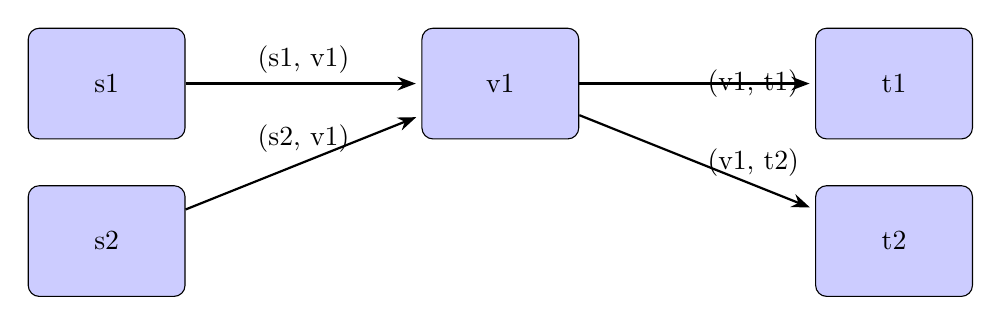
\begin{tikzpicture}[node distance=2cm]

\node[block] (s1) {s1};
\node[block] (s2) [below of=s1] {s2};
\node[block] (v1) [right of=s1, xshift=3cm] {v1};
\node[block] (t1) [right of=v1, xshift=3cm] {t1};
\node[block] (t2) [below of=t1] {t2};

\path[line] (s1) -- node[above] {(s1, v1)} (v1);
\path[line] (s2) -- node[above] {(s2, v1)} (v1);
\path[line] (v1) -- node[right] {(v1, t1)} (t1);
\path[line] (v1) -- node[right] {(v1, t2)} (t2);

\end{tikzpicture}
\end{document}